\section{Codice}
Il codice del progetto è stato organizzato nella sottocartella \texttt{python\_file}, che contiene i seguenti moduli:
\begin{itemize}
    \item Il file \texttt{dataclass} definisce le classi e le trasformazioni per la gestione del dataset di segnali stradali. In particolare, include le classi per l'addestramento (\texttt{StreetSignDataset}) e per il test (\texttt{StreetSignTest}), oltre a trasformazioni quali ridimensionamento (\texttt{Rescale}), ritaglio casuale (\texttt{RandomCrop}), ritaglio specifico (\texttt{Crop}) e conversione in tensori (\texttt{ToTensor}). È inoltre presente la funzione \texttt{show\_landmarks\_batch}, utilizzata per visualizzare batch di immagini con i relativi \textit{landmarks}. Nel complesso, il modulo fornisce l'infrastruttura necessaria alla preparazione dei dati.
    \item Il file \texttt{function} raccoglie le funzioni principali per addestramento e test del classificatore. La prima parte del codice esegue l'addestramento mediante \textit{Stochastic Gradient Descent} e \textit{Cross Entropy Loss}, con supporto a TensorBoard e salvataggio dei pesi. La seconda parte valuta il modello sul set di test, restituendo predizioni ed etichette reali. Nello stesso file sono inoltre presenti le funzioni per l'esportazione dei risultati in formato JSON/CSV e per la generazione dei grafici di accuratezza e loss. È infine inclusa una funzione per il calcolo e la visualizzazione della curva ROC a partire da etichette e predizioni.
    \item Il file \texttt{network} implementa le architetture di rete neurale testate, includendo diverse varianti e l'impiego di tecniche quali \textit{Batch Normalization} e \textit{Dropout}, utili a migliorare prestazioni e capacità di generalizzazione.
    \item Il file \texttt{detect\_and\_classify} implementa la procedura per applicare YOLO al riconoscimento dei segnali stradali in immagini di scenario reale. L'immagine viene inizialmente analizzata da YOLO (addestrato su immagini reali) per individuare il segnale; la porzione ritagliata viene quindi fornita alla rete \textbf{MiniAlexNetV2} per la classificazione. Il sistema realizza così una pipeline completa di \textit{detection} e \textit{classification}.
\end{itemize}

Infine, sono stati creati alcuni notebook in Jupyter, nei quali è stata utilizzata la struttura dati definita in precedenza insieme alle funzioni di training e test, al fine di addestrare il modello. Prima dell'addestramento, le immagini vengono convertite nel formato richiesto dalla struttura dati e sottoposte alle opportune trasformazioni. I notebook realizzati sono i seguenti:
\begin{itemize}
    \item I notebook con intestazione \textit{train} si occupano dell'addestramento delle reti \textit{AlexNet}, \textit{MiniAlexNet} e \textit{MiniAlexNetV2}. In particolare, il notebook esegue il caricamento delle immagini, la loro conversione in tensori e l'addestramento dei modelli, salvando i dati di accuratezza e loss per ogni epoca. Al termine dell'addestramento, i pesi dei modelli vengono salvati per essere successivamente utilizzati nei notebook di \textit{test}, \textit{result} e \textit{graphs}.
    \item \textit{graphs}: carica i dati di accuratezza e loss salvati nei notebook di addestramento e genera i grafici corrispondenti (Loss, Accuracy e ROC).
    \item \textit{result}: carica i tre modelli precedentemente addestrati ed esegue una previsione a partire da un'immagine fornita tramite URL oppure da un'immagine locale. Il notebook restituisce quindi la classe predetta del segnale stradale, tra cui \textit{indicatory} (indicazione), \textit{prohibitory} (divieto) e \textit{warning} (pericolo). In caso di errore nella previsione, viene visualizzato il messaggio \textit{ERROR 404 NOT FOUND}. La classe \textit{Background}, sebbene presente nella fase di addestramento, non viene considerata in quanto non rilevante ai fini dell'applicazione.
    \item \textit{test\_reale}: carica esclusivamente il modello \textit{MiniAlexNetV2} e lo utilizza per eseguire la previsione della categoria del segnale stradale presente in un'immagine reale. In questo caso, l'immagine viene prima elaborata per individuare e ritagliare il segnale stradale, che viene successivamente passato alla rete \textit{MiniAlexNetV2} per la classificazione. La classe predetta viene quindi sovrapposta all'immagine, che viene infine visualizzata.
\end{itemize}

\subsection{Caso Reale}
Analizziamo più in dettaglio il notebook \textit{test\_reale} in cui è presente la parte di codice relativa al test della rete neurale in un contesto urbano. Se, per esempio, dotassimo un veicolo di una telecamera per riprendere la strada in tempo reale, potremmo acquisire delle immagini durante il tragitto e verificare la presenza di segnali stradali, inviando infine l'output al sistema di bordo o al guidatore. Per fare ciò, ci si è posti il problema di come isolare la singola immagine del segnale rispetto al contesto. Per eseguire questa ricerca sono stati studiati due processi:

\begin{itemize}
    \item \textbf{Divisione in sottoimmagini:} consiste nel suddividere l'immagine in numerose porzioni e verificare per ognuna di esse se contiene un segnale stradale.
    \item \textbf{Uso di YOLO:} utilizzo di uno strumento di object detection che permette di individuare le regioni d'interesse (ROI) all'interno delle immagini, identificando le porzioni candidate alla classificazione.
\end{itemize}

\subsubsection{Divisione}
L'uso della divisione in sottoimmagini è la soluzione più semplice, ma ha presentato scarsi risultati sia in termini di prestazioni che di affidabilità. Il motivo risiede nella necessità di processare sequenzialmente ogni ritaglio, causando lentezza di calcolo. Inoltre, l'accuratezza è limitata dal fatto che il dataset di addestramento non copre tutte le possibili variazioni del contesto circostante. Si aggiunge poi il problema del ritaglio: quando si esegue il taglio dell'immagine, il segnale non sempre ricade al centro della sottoimmagine e può risultare solo parziale. Questo fa sì che la rete non sia in grado di riconoscere il segnale oppure produca falsi positivi.

\subsubsection{YOLO}
Per ovviare ai limiti della suddivisione manuale, nel notebook \textit{test\_reale} è stato implementato l'uso dell'algoritmo \textbf{YOLO} (You Only Look Once). A differenza dell'approccio precedente, YOLO esegue l'object detection in un unico passaggio, identificando istantaneamente le coordinate dei segnali stradali (\textit{Bounding Boxes}) all'interno di scene complesse, per poi passare la porzione d'immagine ritagliata contenente il segnale alla rete \textit{MiniAlexNetV2} per identificarne la tipologia.

Il flusso di lavoro implementato prevede i seguenti passaggi:
\begin{enumerate}
    \item Caricamento dell'immagine ad alta risoluzione catturata nel contesto urbano.
    \item Applicazione del modello YOLO per individuare le regioni d'interesse (ROI) corrispondenti ai segnali.
    \item Ritaglio (\textit{cropping}) automatico delle aree individuate.
    \item Passaggio dei ritagli alla rete \textbf{MiniAlexNetV2} per la classificazione finale della macro-categoria.
\end{enumerate}

Questo approccio ibrido ha permesso di ottenere una precisione estremamente elevata, poiché la rete di classificazione lavora solo su porzioni di immagine già identificate come "segnali", eliminando il rumore di fondo del contesto cittadino e riducendo drasticamente i tempi di calcolo rispetto alla scansione sequenziale.

\subsubsection{Analisi dei Risultati}
Una volta spiegati i vari metodi, si procede a visualizzare la differenza tra i due approcci utilizzati. Prima nel caso di utilizzo di un'immagine presa dalle immagini di test (Figura \ref{fig:test1}) con cui abbiamo addestrato la rete: possiamo notare che, nel caso dell'algoritmo di \textbf{divisione}, abbiamo ottenuto dei falsi positivi e, inoltre, alcune porzioni di immagine, essendo state ritagliate in modo non perfetto, sono state classificate erroneamente. Per quanto riguarda l'uso di \textbf{YOLO}, invece, si è avuta l'identificazione di un solo segnale, che è stato poi classificato correttamente dalla rete \textit{MiniAlexNetV2}, ma non ha identificato gli altri segnali presenti.

\begin{figure}[htbp]
\centering
\begin{subfigure}[t]{0.50\textwidth}
    \centering
    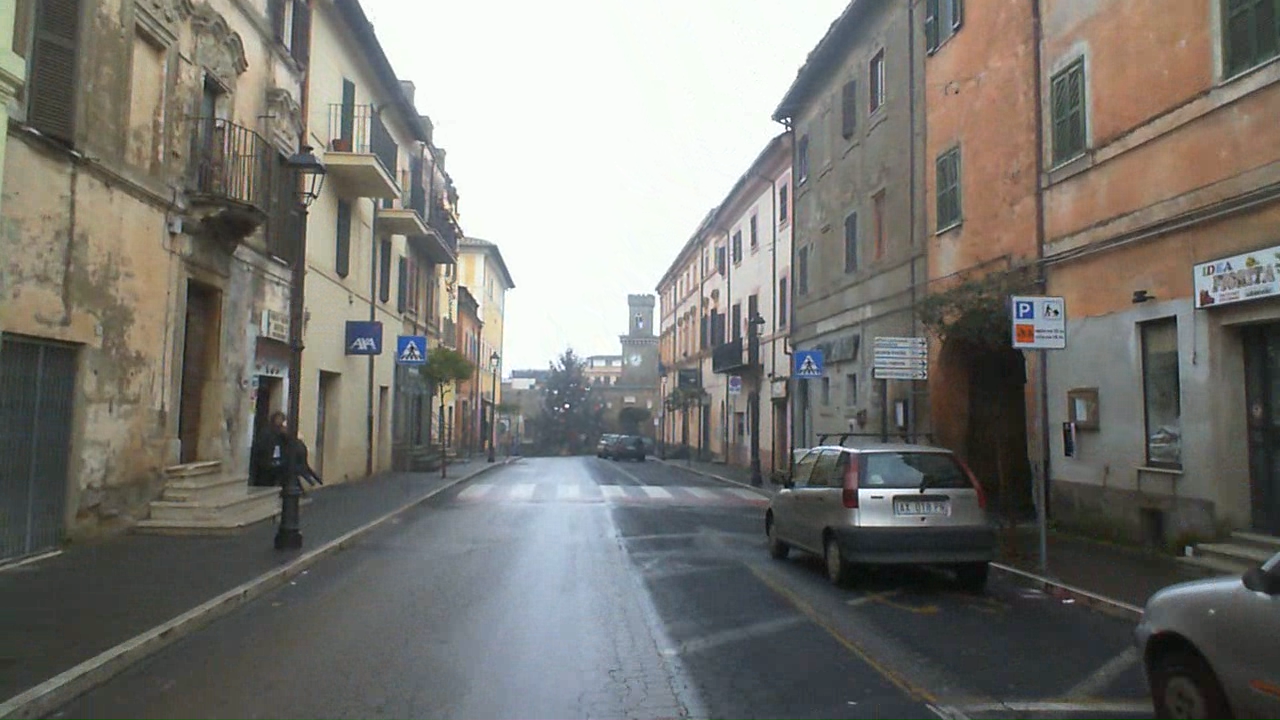
\includegraphics[width=0.9\linewidth]{Codice/test2.png}
    \caption{Immagine originale}
\end{subfigure}\hfill
\begin{subfigure}[t]{0.50\textwidth}
    \centering
    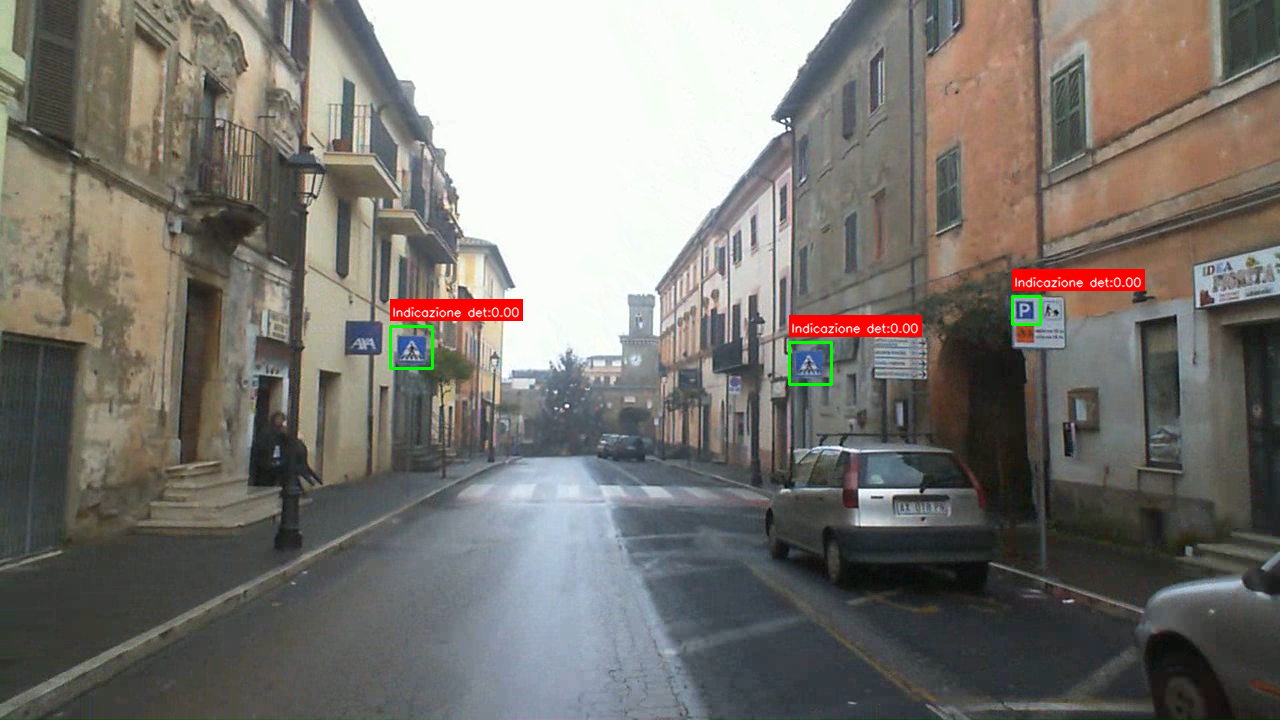
\includegraphics[width=0.9\linewidth]{Codice/test2_std.png}
    \caption{Immagine originale con label}
\end{subfigure}
\vfill
\begin{subfigure}[t]{0.50\textwidth}
    \centering
    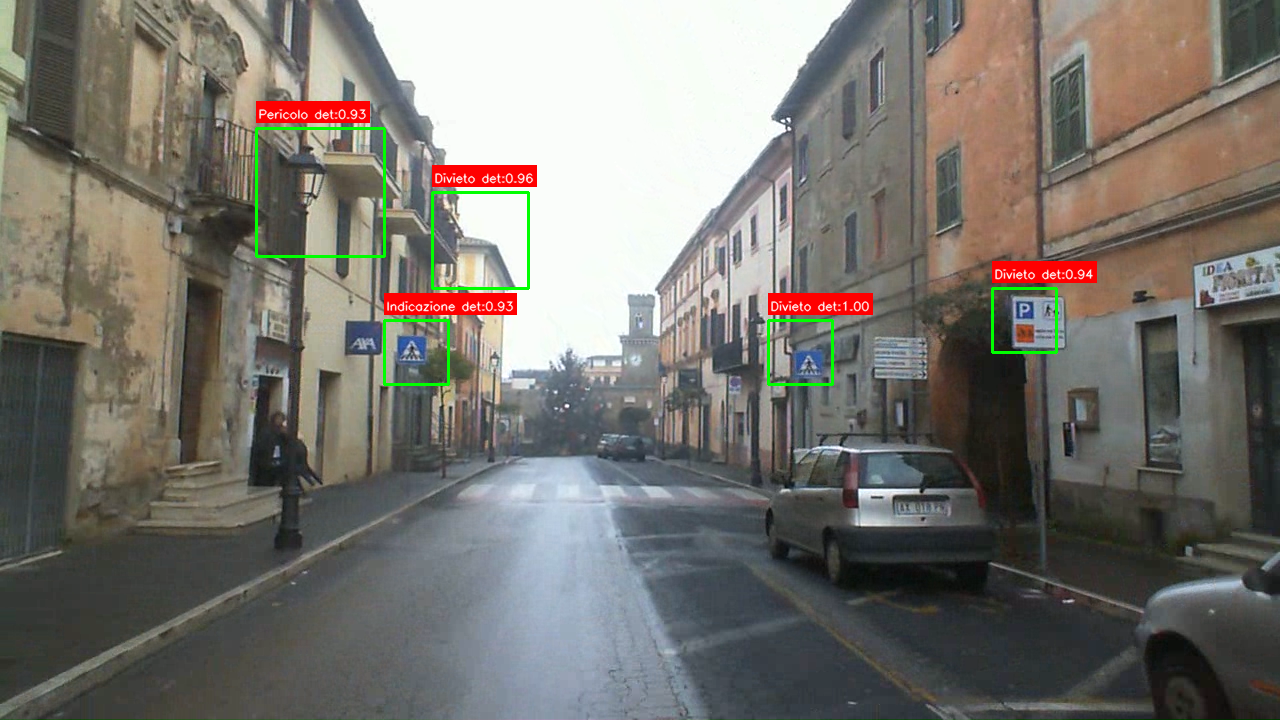
\includegraphics[width=0.9\linewidth]{Codice/test2_div.png}
    \caption{Divisione}
\end{subfigure}\hfill
\begin{subfigure}[t]{0.50\textwidth}
    \centering
    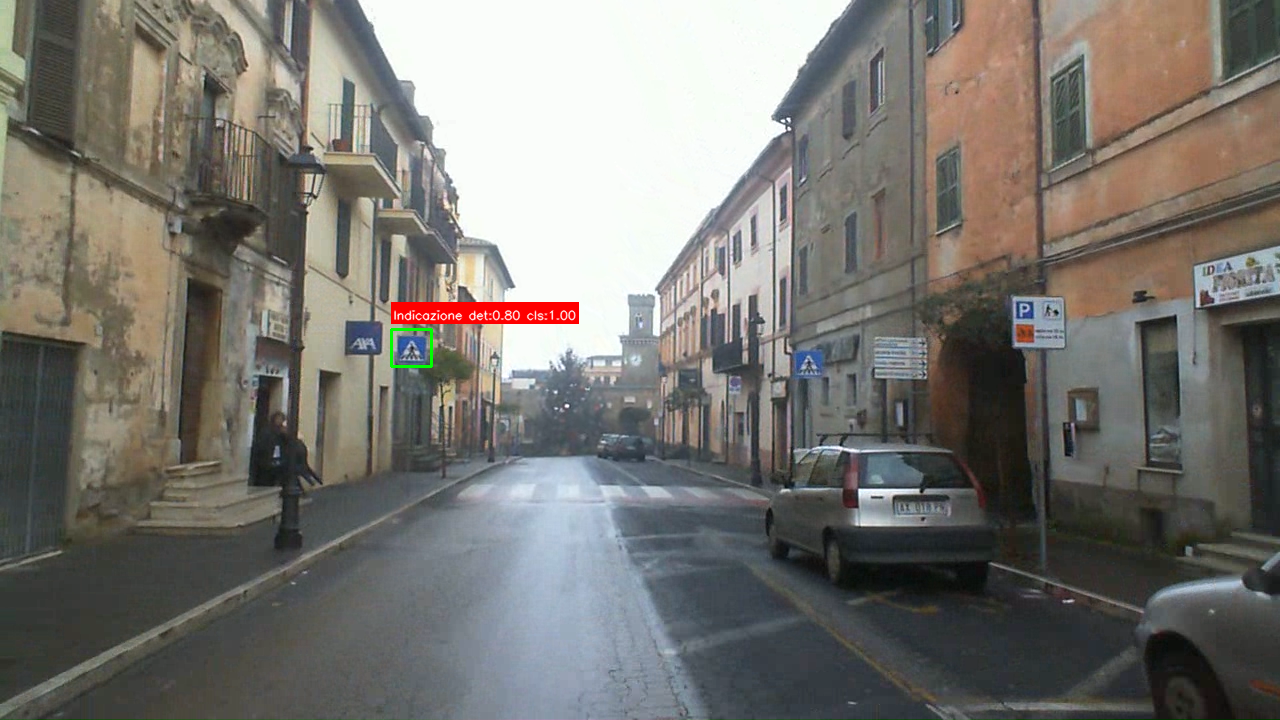
\includegraphics[width=0.9\linewidth]{Codice/test2_yolo.png}
    \caption{YOLO}
\end{subfigure}
\caption{Confronto tra i metodi di divisione e YOLO su un'immagine del dataset di test.}
\label{fig:test1}
\end{figure}

Per quanto riguarda invece il caso in cui viene usata un'immagine campione casuale presa online (Figura \ref{fig:test2}), possiamo notare che \textbf{YOLO} si è comportato meglio rispetto all'algoritmo di \textbf{divisione}, poiché quest'ultimo ha eseguito dei tagli che talvolta risultavano superflui.

\begin{figure}[htbp]
\centering
\begin{subfigure}[t]{0.33\textwidth}
    \centering
    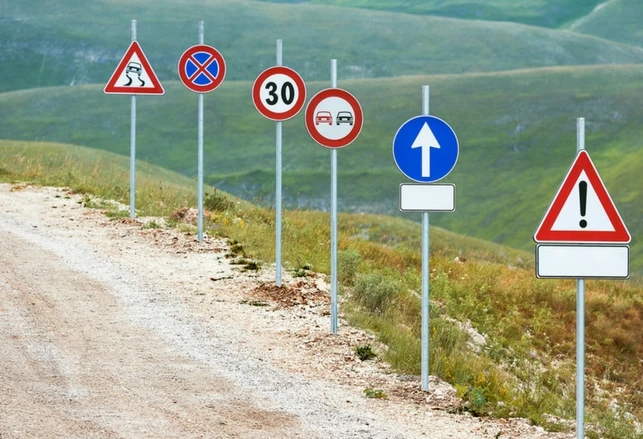
\includegraphics[width=0.9\linewidth]{Codice/test1.png}
    \caption{Immagine originale}
\end{subfigure}\hfill
\begin{subfigure}[t]{0.33\textwidth}
    \centering
    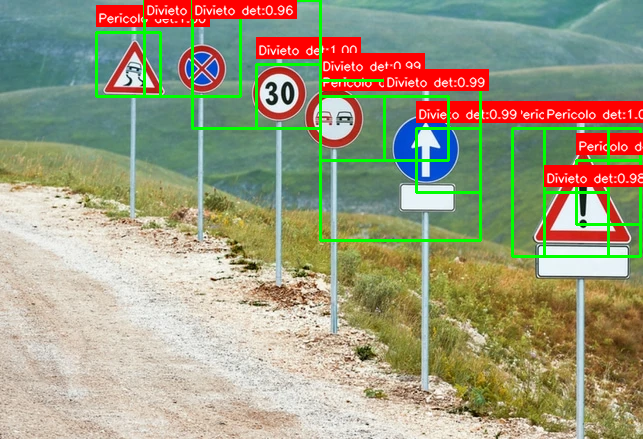
\includegraphics[width=0.9\linewidth]{Codice/test_div1.png}
    \caption{Divisione}
\end{subfigure}\hfill
\begin{subfigure}[t]{0.33\textwidth}
    \centering
    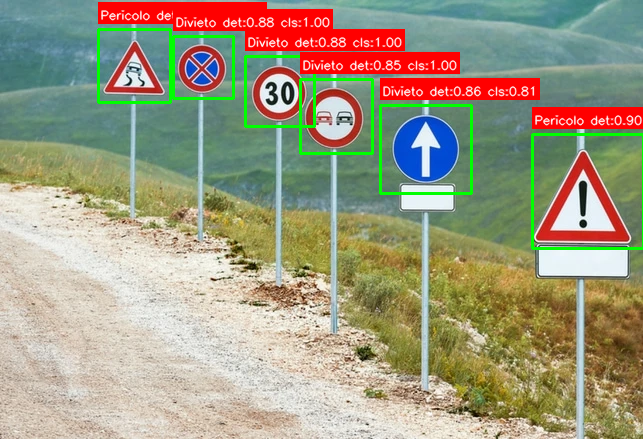
\includegraphics[width=0.9\linewidth]{Codice/test_yolo1.png}
    \caption{YOLO}
\end{subfigure}
\caption{Confronto tra i metodi di divisione e YOLO su un'immagine casuale.}
\label{fig:test2}
\end{figure}

In sintesi, nessuno dei due metodi si è rivelato perfetto nell'analisi di un contesto reale, ma entrambi possono essere utilizzati come punto di partenza per comprendere come procedere.